\chapter{Experimental setup}
Experiments were executed on variations of the \textit{Cart-pole} environment and on variations of the \textit{Acrobot} environment.\\

\section{Cart-pole environment} % (fold)
\label{sub:cartpole_environment}
In the 2-dimensional Cart-pole environment, a pole is placed vertically on a cart.
The goal in this environment is to keep the pole balanced vertically (i.e. keep the angle of the pole between thresholds) and to keep the cart between 2 borders.
The state is defined by 4 continuous-valued attributes: the position of the cart, the velocity of the cart, the angle of the pole and the angular velocity of the pole.
A discrete value of $1$ is given as a reward each time the pole is balanced and the cart is between bounds.
The episode ends either when these requirements are not fulfilled anymore or 200 steps have been executed.
An agent can either move left or right. It can't stay at its current position.
The environment is visualized in Figure~\ref{fig:cartpole}.
\begin{figure}[htb]
    \centering
    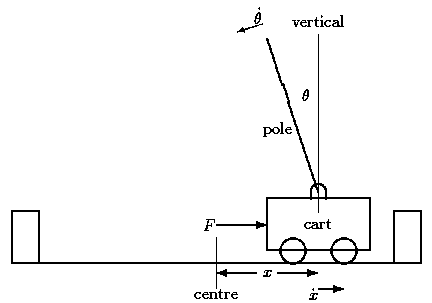
\includegraphics[width=.6\linewidth]{images/cartpole.png}
    \caption[Cart-pole environment]{Cart-pole environment. $F$ is the force applied to the cart when taking an action. $x$ is the distance of the cart from the center and $\dot{x}$ is its velocity. $\theta$ is the angle of the pole and $\dot{\theta}$ refers to its angular velocity. Source: \cite{grant1990modelling}.}
    \label{fig:cartpole}
\end{figure}
For executing the experiments, an implementation of this environment by \cite{Brockman2016OpenAIGym} was used.\\
% section cartpole_environment (end)

\section{Acrobot environment} % (fold)
\label{sub:acrobot_environment}
The goal in the \textit{Acrobot} environment, visualized in Figure~\ref{fig:acrobot} is to swing up  the tip of 2 joined arms above a certain point \cite{spong1995swing}.
This can be done by applying a force on the joint between the 2 arms.
However, this force is not enough to fulfill the goal immediately. Instead, the actuator must apply force to the left and to the right to build up enough speed to get above the horizontal threshold.
The state consists of the angle and angular velocity of both arms. One can either move the joint clockwise, counter-clockwise or do nothing.
An episode stops either when the tip of the outermost arm is above the threshold or when 500 steps have been executed in the episode.
The goal is to minimize the amount of steps necessary to reach the threshold.
\begin{figure}[htb]
    \centering
    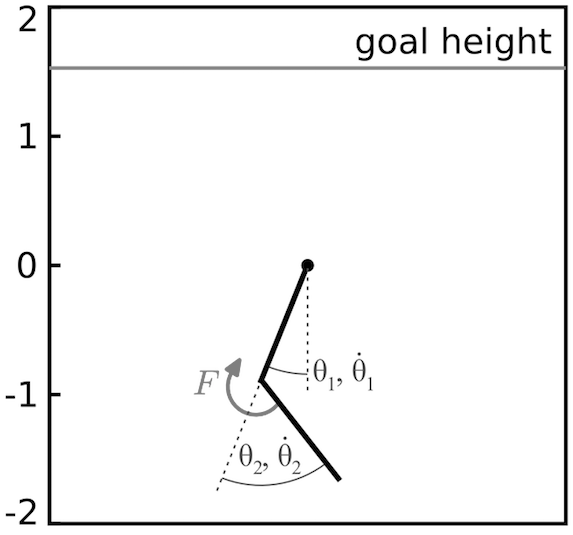
\includegraphics[width=.7\linewidth]{images/acrobot.png}
    \caption[Acrobot environment]{Acrobot environment. $\theta_1$ and $\dot{\theta_1}$ are respectively the angle and angular velocity of the arm attached to the central fixed point. $\theta_2$ and $\dot{\theta_2}$ are respectively the angle and angular velocity of the outermost arm. Source: \cite{fremaux2013reinforcement}}
    \label{fig:acrobot}
\end{figure}
% section acrobot_environment (end)

\section{Methodology} % (fold)
\label{sub:methodology}
Several experiments were executed, depending on the algorithm, the environment, the number of source tasks and which knowledge was transferred to the target task.\\

In the first experiment, first a number of environments are randomly generated. We try to learn with both 5 and 10 environments.
The environment for each task can differ for a predefined number of attributes, of which the values can each be in a certain range. For a cart-pole task, these are the mass of the cart, the mass of the pole and the length of the pole.\\
Then a number of source tasks are learned that can update both the shared knowledge base and their own sparse representation.
After a number of epochs, i.e. updates to these variables, we stop with learning these tasks.
Instead, we learn to solve a new task, the target task, for which we hadn't learned its sparse representation yet. Here however, only the sparse representation can be updated and not the shared knowledge base.\\

In the second experiment, besides transferring the shared knowledge base, a sparse representation was also transferred.
This is a sparse representation randomly chosen from the source tasks.
The target task can then change this sparse representation to improve the performance on its own problem instance.\\

The last experiment involves the \textit{REINFORCE} algorithm and was used as comparison with the results of the other experiments.
Here, we first run the algorithm on one source task then transfer the same knowledge to the target task.
In practice, this means that we start learning on the target task with the weights learned using the source task.
The algorithm can still learn adapt all the weights using the target task.
No sparseness on the weights was enforced.\\

All three experiments were executed on the cart-pole and acrobot environment.
Each experiment consisted of 100 runs, each time using a different set of environments and thus problems to solve.\\
Afterwards the rewards are averaged over all the runs.\\
Trajectories for both sets of tasks contained of maximally 200 or 500 steps depending on the type of environment.
This could be less in case the environment was in an end state.
In case of the cart-pole environment, this can mean for example that the cart tried to cross the left or right border or that the pole fell down.\\
Hyperparameters, such as the learning rate of neural networks, were chosen by iteratively executing the previously mentioned experiment. Possible values for each hyperparameter were chosen manually.
% section methodology (end)

\section{Results}
\todo{Add with more experiments}
To evaluate our proposed algorithm, we use different experiments. First we compare the sequential and parallel version of our algorithm. Afterwards, we see if transferring a sparse representation from a random source task to the target task yields improvements.
When discussing the jumpstart and asymptotic performance, we use the mean reward at respectively the first 5 and the last 5 epochs (updates to the artificial neural network parameters).

\subsection{Parallel and sequential knowledge transfer} % (fold)
\label{sub:parallel_and_sequential_knowledge_transfer}
We first compare the performance of the algorithm that learns the source tasks in parallel with the one that learns them sequentially. We do this for the cart-pole environment in order to determine which version of the algorithm to use for further experiments.

The performance of both versions of the algorithm and for both the source tasks and target task is shown in Figure~\ref{fig:CartPole:reward_akt-kt_all_5tasks}.
\begin{figure}[htb]
    \centering
    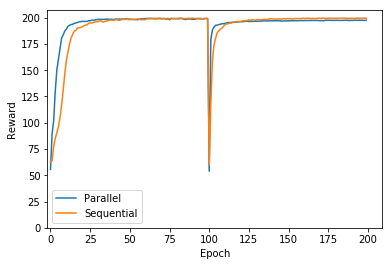
\includegraphics[width=.8\linewidth]{images/results/CartPole/kt_akt/reward_source-target_5tasks.png}
    \caption[Learning curves for the parallel and sequential version of our algorithm applied to the \textit{cart-pole} environment]{Learning curves for the parallel and sequential version of our algorithm applied to the \textit{cart-pole} environment. Until epoch 100, the mean performance on the source tasks is shown. Afterwards, the performance on the target task is shown.}
    \label{fig:CartPole:reward_akt-kt_all_5tasks}
\end{figure}
Here, we see that, on average, the parallel version of our algorithm converges faster than the sequential version.
To find out which version is better, we first compare the median of the area under curve (AUC) over all the runs.
For the sequential version, the AUC is $19446.096$, while it is $19655.268$ for the parallel version.
We now use a Wilcoxon rank-sum test with the null-hypothesis that there is no.
We get $W=8.244$ and $1.665*10^{-16}$.
With a significance level of $0.05$, we can reject the null-hypothesis and say that the medians of the 2 versions are different.
By observing those medians, we can say that the parallel version is better.\\
For the following experiments, when referring to "our transfer learning algorithm", the parallel version will be used.
% subsection parallel_and_sequential_knowledge_transfer (end)

\subsection{Feature extraction} % (fold)
\label{sub:feature_extraction}
In this experiment, we evaluate the use of feature extraction on the states. We compare the performance of an artificial neural network with a layer of 5 units, one with 10 units and one without feature extraction at all. The learning curves for the performance on the target task are shown in Figure~\ref{fig:CartPole:feature_extraction}.
\begin{figure}[htb]
    \centering
    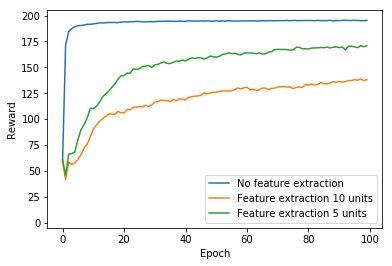
\includegraphics[width=.8\linewidth]{images/results/CartPole/feature_extraction.png}
    \caption{Caption}
    \label{fig:CartPole:feature_extraction}
\end{figure}
Feature extraction does not seem to improve the performance of the algorithm for this environment. It only seems to slow down learning. It is worse when we use more units in the hidden layer used for feature extraction. As more units are added, more weights influence the result and more of these weights must be learned.\\
It must be noted however that for algorithms working with high-dimensional inputs, feature extraction, using for example deep learning, is necessary to obtain a good performance. In this environment, the state contains values that are useful for solving a task. However, without feature extraction, it is not clear if a certain pixel of an image is important. Feature extraction is able to obtain values relevant for solving the task.
% subsection feature_extraction (end)

\subsection{Without sparse representation transfer} % (fold)
\label{sub:cartpole:without_sparse_representation_transfer}
We now explore the differences between learning directly on a target task and first learning on source tasks (i.e. using our transfer learning algorithm), using the metrics that we defined in Section~\ref{sub:tl_metrics}.
We consider both 5 and 10 source tasks.
The algorithms using 5 source tasks and 10 source tasks are referred to as respectively \textit{TLA 5} and \textit{TLA 10}.
For the regular algorithm, we use the \textit{REINFORCE} that was discussed in Section~\ref{sub:rl_policy_gradient}.

\subsubsection{Cart-pole} % (fold)
\label{ssub:without_sparse_representation_transfer:cartpole}
The learning curve of both algorithms on the target task is visualized in Figure~\ref{fig:CartPole:reward_target_re-akt5-akt10}.
\begin{figure}[htb]
    \centering
    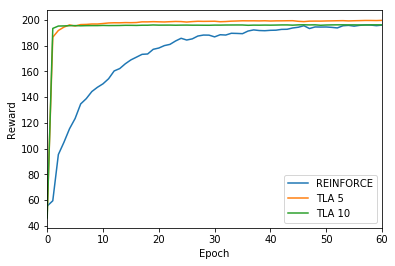
\includegraphics[width=.8\linewidth]{images/results/CartPole/no_sparse_transfer/reward_target_re-akt5-akt10.png}
    \caption[Learning curves for \textit{REINFORCE} and \textit{TLA} for the \emph{Cart-pole} environment]{Learning curves for the \textit{Cart-pole} environment of the \textit{REINFORCE} algorithm and our transfer learning algorithm (\textit{TLA}) with 5 source tasks (shown as \textit{TLA 5}) and 10 source tasks (shown as \textit{TLA 10}). The learning curves are only shown until epoch 60 in order to better show the initial performance of the algorithms. All the algorithms converged and achieved the same rewards after this epoch.}
    \label{fig:CartPole:reward_target_re-akt5-akt10}
\end{figure}
It can be seen visually that, on average, in all the configurations the jumpstart performance is about the same. We now compare the means, standard deviations and the medians of the jumpstart performances of the algorithms. This is shown in Table~\ref{tab:cartpole:nosparse:stats}.
\begin{table}[htb]
    \centering
    \begin{tabular}{llccc}
    \hline
    Algorithm & Mean & Standard deviation & Median \\
    \hline
       REINFORCE  & $86.060$ & $25.330$ & $86.886$ \\
       \textit{TLA 5} & $158.237$ & $23.153$ & $163.840$ \\
       \textit{TLA 10} & $\bm{165.120}$ & $\bm{21.955}$ & $\bm{169.034}$ \\
    \hline
    \end{tabular}
    \caption{Mean, standard deviation and median of the jumpstart performances for \textit{REINFORCE}, \textit{TLA 5} and \textit{TLA 10} applied to the cart-pole environment.}
    \label{tab:cartpole:nosparse:stats}
\end{table}
It can be seen that the best jumpstart performance is achieved using \textit{TLA 10}, as it has the highest mean and median and varies the least. As it learned on more source tasks, it has more samples from the distribution of environment parameters and thus it can cover more kinds of task variations. \textit{REINFORCE} performs the worst, as it must learn without any prior learned knowledge.\\

We can also see in Figure~\ref{fig:CartPole:reward_target_re-akt5-akt10} that \textit{REINFORCE} takes longer on average to reach the maximum reward (which is $200$ in this environment). As a result, the area under curve for \textit{REINFORCE} is $18170.243$ whereas it is $19130.824$ and $19329.318$ for respectively \textit{TLA 5} and \textit{TLA 10}.\\
In every configuration, the maximum reward ($200$) is reached eventually and as such they have the same asymptotic performance.\\

\subsubsection{Acrobot} % (fold)
\label{ssub:without_sparse_representation_transfer:acrobot}
We will do with the same experiment as in Section~\ref{ssub:without_sparse_representation_transfer:cartpole}, but with the \textit{Acrobot} environment.
As can be seen in Figure~\ref{fig:Acrobot:reward_target_re-akt5-akt10}, the average performance of the \textit{REINFORCE} algorithm on the target task is different from \textit{TLA 5} and \textit{TLA 10}.
\begin{figure}[htb]
    \centering
    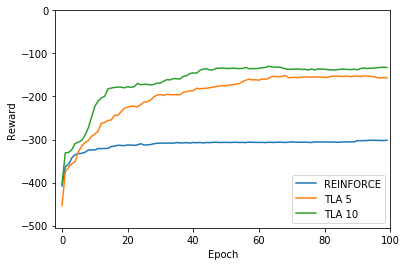
\includegraphics[width=.8\linewidth]{images/results/Acrobot/no_sparse_transfer/reward_target_re-akt5-akt10.png}
    \caption[Learning curves for the \textit{Acrobot} environment of \textit{REINFORCE} and \textit{TLA} for the \emph{Acrobot} environment]{Learning curves of the \textit{REINFORCE} algorithm and our transfer learning algorithm (\textit{TLA}) with 5 source tasks (shown as \textit{TLA 5}) and 10 source tasks (shown as \textit{TLA 10}).}
    \label{fig:Acrobot:reward_target_re-akt5-akt10}
\end{figure}
We will now discuss how exactly the behavior of these algorithms differ, starting by looking at the jumpstart performances. Statistics of the jumpstart performances are shown in Table~\ref{tab:acrobot:nosparse:stats}.
\begin{table}[htb]
    \centering
    \begin{tabular}{llccc}
    \hline
    Algorithm & Mean & Standard deviation & Median \\
    \hline
       \textit{REINFORCE}  & $-361.209$ & $\bm{159.760}$ & $-490.063$ \\
       \textit{TLA 5} & $-380.222$ & $160.589$ & $-500.000$ \\
       \textit{TLA 10} & $\bm{-339.530}$ & $168.845$ & $\bm{-419.571}$ \\
    \hline
    \end{tabular}
    \caption{Mean, standard deviation and median of the jumpstart performances for \textit{REINFORCE}, \textit{TLA 5} and \textit{TLA 10} applied to the Acrobot environment.}
    \label{tab:acrobot:nosparse:stats}
\end{table}
We see that \textit{TLA 10} performs the best. However, as seen by the standard deviations, the results can differ considerably. We will see if the differences in medians are significant by using a Wilcoxon rank-sum test with for each pair of algorithms the null-hypothesis that there is no difference between them.
The resulting p-values are shown in Table~\ref{tab:sparse:pvalues}.
\begin{table}[htb]
    \centering
    \begin{tabular}{llccc}
    \hline
    Algorithm & \textit{REINFORCE} & \textit{TLA 5} & \textit{TLA 10} \\
    \hline
       \textit{REINFORCE}  & & & \\
       \textit{TLA 5} & $0.512$ & & \\
       \textit{TLA 10} & $0.426$ & $0.179$ & \\
    \hline
    \end{tabular}
    \caption{P-values for the Wilcoxon rank-sum test of the jumpstart performances using different algorithms, applied to the Acrobot environment, where the \textit{TLA} algorithms use sparse representation transfer.}
    \label{tab:sparse:pvalues}
\end{table}
We can say using each time a significance level of $0.05$ that there is no difference between any combination of algorithms.\\

As we could already see in Figure~\ref{fig:Acrobot:reward_target_re-akt5-akt10}, the learning performance of the \textit{REINFORCE} algorithm seems to be lower on average than the other algorithms.
This is also visible when looking at the area under curve, which is $-30810.360$ for \textit{REINFORCE} algorithm and $-19437.733$ and $-16223.803$ for respectively \textit{TLA 5} and \textit{TLA 10}.\\

Last, we compare the asymptotic performances, again with the same test and the null-hypotheses that there are no differences between the asymptotic performances. The resulting p-values are shown in Table~\ref{tab:sparse:asymp:pvalues}.
\begin{table}[htb]
    \centering
    \begin{tabular}{llccc}
    \hline
    Algorithm & \textit{REINFORCE} & \textit{TLA 5} & \textit{TLA 10} \\
    \hline
       \textit{REINFORCE}  & & & \\
       \textit{TLA 5} & $1.034*10^{-4}$ & & \\
       \textit{TLA 10} & $7.091*10^{-6}$ & $0.449$ & \\
    \hline
    \end{tabular}
    \caption{P-values for the Wilcoxon rank-sum test using different algorithms where the \textit{TLA} algorithms use sparse representation transfer.}
    \label{tab:sparse:asymp:pvalues}
\end{table}

With a significance level of $0.05$, we can say that there is a difference between \textit{REINFORCE} and \textit{TLA 5} and between \textit{REINFORCE} and \textit{TLA 10}.
With the same significance level, we retain the null-hypothesis for \textit{TLA 5} and \textit{TLA 10}.
Thus, we can say that using knowledge transfer yields a significant difference in the resulting performance, when applied to the Acrobot environment.
To further discuss these differences, we look at the boxplots of the asymptotic performances for the three configurations. These are shown in Figure~\ref{fig:Acrobot:asymp_target_re-akt5-akt10}.
\begin{figure}[htb]
    \centering
    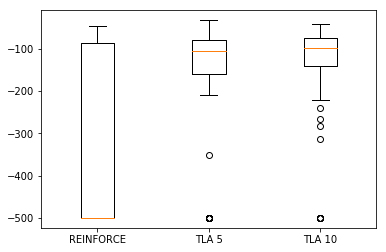
\includegraphics[width=.8\linewidth]{images/results/Acrobot/no_sparse_transfer/asymp_target_re-akt5-akt10.png}
    \caption{Boxplots of the asymptotic performances of \textit{REINFORCE}, \textit{TLA 5} and \textit{TLA 10} using the \textit{Acrobot} environment.}
    \label{fig:Acrobot:asymp_target_re-akt5-akt10}
\end{figure}
We can see that the median for the \textit{REINFORCE} algorithm is still the lowest possible reward for this environment. This means that in half of the cases, the \textit{REINFORCE} algorithm cannot improve and cannot get past the minimum reward. The medians of \textit{TLA 5} and \textit{TLA 10} are respectively $-105.305$ and $-98.391$. Only some outliers of these algorithms don't get past the minimum reward.
% subsubsection acrobot (end)

% To further explore the jumpstart performance, we will look at boxplots of the jumpstarts of both algorithms, computed using all the 100 runs of both algorithms. These are shown in Figure~\ref{fig:boxplot_tla_re_5envs}.
% \begin{figure}[htb]
%     \centering
%     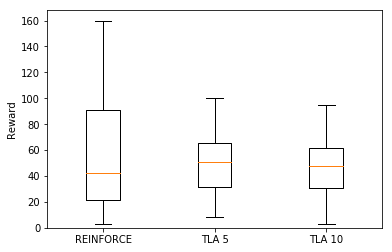
\includegraphics[width=.8\linewidth]{images/results/CartPole/no_sparse_transfer/jumpstart_target_re-akt5-akt10.png}
%     \caption{Boxplot of the jumpstart performance of \textit{REINFORCE} and our transfer learning algorithm (\textit{TLA}).}
%     \label{fig:boxplot_tla_re_5envs}
% \end{figure}
% We can see that, although the mean jumpstart performances are different, there is little difference between the medians: $22.774$ for \textit{REINFORCE} and $23.459$ for our algorithm. However, our algorithm is able to reach a higher initial performance more often. In 75\% of the cases, the jumpstart performance for \textit{REINFORCE} is below $55.535$, while it is $160.595$ for our algorithm.

% subsubsection cartpole:without_sparse_representation_transfer (end)
\subsection{With sparse representation transfer} % (fold)
\label{sub:cartpole:with_sparse_representation_transfer}
We now explore the results of transferring a sparse representation. After learning on the source tasks, we initialize the sparse representation weights with those of a randomly chosen sparse representation of a source task. The algorithm can then change this sparse representation to improve its performance on the target task. We compare the results to those when not transferring the sparse representation, both for the cart-pole and the acrobot environment.
\subsubsection{Cart-pole} % (fold)
\label{ssub:with_sparse_representation_transfer:cartpole}
To see how both version of the algorithm differ on average in terms of learning performance, we take a look at the learning curves, which are shown in Figure~\ref{fig:CartPole:st:reward_target_without-with}.
\begin{figure}[htb]
    \centering
    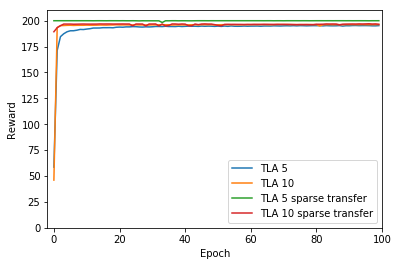
\includegraphics[width=.8\linewidth]{images/results/CartPole/sparse_transfer/reward_target_without_with.png}
    \caption[Learning curves for the \textit{Cart-pole} environment of \textit{TLA} with and without sparse representation transfer]{Learning curves for the \emph{Cart-pole} environment of our transfer learning algorithm (\textit{TLA}) with 5 source tasks (shown as \textit{TLA 5}) and 10 source tasks (shown as \textit{TLA 10}), both with and without sparse representation transfer.}
    \label{fig:CartPole:st:reward_target_without-with}
\end{figure}
It can be seen that the versions using sparse representation transfer need little to no update to reach the maximum reward. However, all versions converge to the maximum as all the medians of the asymptotic performances are $200$.

We now compare the jumpstart performances of these algorithms using statistics, shown in Table~\ref{tab:cartpole:sparse:jumpstart:stats}.
\begin{table}[htb]
    \centering
    \begin{tabular}{llccc}
    \hline
    Algorithm & Sparse repr. transfer & Mean & Standard deviation & Median \\
    \hline
       \textit{TLA 5} & No & $158.237$ & $23.153$ & $163.840$ \\
       \textit{TLA 10} & No & $165.120$ & $21.955$ & $169.034$ \\
       \textit{TLA 5} & Yes & $\bm{199.997}$ & $0.0220$ & $\bm{200.000}$ \\
       \textit{TLA 10} & Yes & $194.260$ & $23.742$ & $\bm{200.000}$ \\
    \hline
    \end{tabular}
    \caption{Mean, standard deviation and median of the jumpstart performances for \textit{TLA 5} and \textit{TLA 10}, with without and with sparse representation transfer, applied to the cart-pole environment.}
    \label{tab:cartpole:sparse:jumpstart:stats}
\end{table}
As shown, the versions using sparse representation transfer perform better initially.
It can be seen in Figure~\ref{fig:CartPole:st:reward_target_without-with}.

% We now determine if the jumpstart performances differ significantly, again using a Wilcoxon rank-sum test with the null-hypothesis that there is no difference. The resulting p-values are shown in
% subsubsection cartpole (end)
\subsubsection{Acrobot} % (fold)
\label{ssub:with_sparse_representation_transfer:acrobot}
To discuss the differences between the 2 versions for the \textit{acrobot} environment, we also look at the learning curves, which are shown in Figure~\ref{fig:Acrobot:st:reward_target_without-with}.
\begin{figure}[htb]
    \centering
    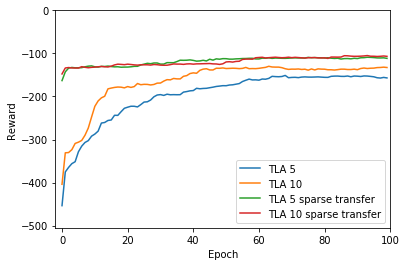
\includegraphics[width=.8\linewidth]{images/results/Acrobot/sparse_transfer/reward_target_without_with.png}
    \caption[Learning curves for the \textit{acrobot} environment of \textit{TLA} with and without sparse representation transfer]{Learning curves for the \emph{acrobot} environment of our transfer learning algorithm (\textit{TLA}) with 5 source tasks (shown as \textit{TLA 5}) and 10 source tasks (shown as \textit{TLA 10}), both with and without sparse representation transfer.}
    \label{fig:Acrobot:st:reward_target_without-with}
\end{figure}
It can be seen that, on average, the version using sparse representation transfer can start with a high reward but improves little afterwards.
However, the rewards stay superior to those using the version without sparse representation transfer.\\

First, we see how the 2 versions perform initially, using the jumpstart performances. Statistics about the jumpstart performances are presented in Table~\ref{tab:acrobot:sparse:stats}.
\begin{table}[htb]
    \centering
    \begin{tabular}{llccc}
    \hline
    Algorithm & Sparse repr. transfer & Mean & Standard deviation & Median \\
    \hline
       \textit{TLA 5} & No & $-380.222$ & $160.589$ & $-500.000$ \\
       \textit{TLA 10} & No & $-339.530$ & $168.845$ & $-419.571$ \\
       \textit{TLA 5} & Yes & $-141.236$ & $101.567$ & $-110.482$ \\
       \textit{TLA 10} & Yes & $\bm{-136.400}$ & $97.188$ & $\bm{-108.157}$ \\
    \hline
    \end{tabular}
    \caption{Mean, standard deviation and median of the jumpstart performances \textit{TLA 5} and \textit{TLA 10} both with and without sparse representation transfer, applied to the Acrobot environment.}
    \label{tab:acrobot:sparse:stats}
\end{table}
Indeed, the versions using sparse representation transfer obtain initially obtain a higher reward and are more stable.\\
Next, we use the same types of statistics for the asymptotic performances.
These are shown in Table~\ref{tab:acrobot:sparse:asymp:stats}.
\begin{table}[htb]
    \centering
    \begin{tabular}{llccc}
    \hline
    Algorithm & Sparse repr. transfer & Mean & Standard deviation & Median \\
    \hline
       \textit{TLA 5} & No & $-156.128$ & $137.661$ & $-107.222$ \\
       \textit{TLA 10} & No & $-132.873$ & $105.777$ & $-96.224$ \\
       \textit{TLA 5} & Yes & $-110.481$ & $67.384$ & $-93.085$ \\
       \textit{TLA 10} & Yes & $\bm{-106.626}$ & $64.108$ & $\bm{-91.087}$ \\
    \hline
    \end{tabular}
    \caption{Mean, standard deviation and median of the asymptotic performances \textit{TLA 5} and \textit{TLA 10} both with and without sparse representation transfer, applied to the Acrobot environment.}
    \label{tab:acrobot:sparse:asymp:stats}
\end{table}
Again, the versions with sparse representation transfer perform better, because a higher mean and median reward is achieved and the standard deviations are lower.\\
Using these statistics, we see that a sparse representation is a useful and more stable starting point for the target task and also leads to a better performance at the end.
We can also notice that the performance is better when using using 10 source tasks instead of 5. To see if this difference is significant, we use a Wilcoxon rank-sum test with the null-hypothesis that there is no difference. This results in a p-value of $0.653$. Thus, with a significance level of $0.05$, we can retain the null-hypothesis and say that the difference in medians is not significant.
% subsubsection acrobot (end)
% subsection with_sparse_representation_transfer (end)

\subsection{REINFORCE using a source and target task} % (fold)
\label{sub:reinforce_using_a_source_and_target_task}
\subsubsection{Cart-pole} % (fold)
\label{ssub:reinforce_source_target:cart_pole}
\begin{figure}[htb]
    \centering
    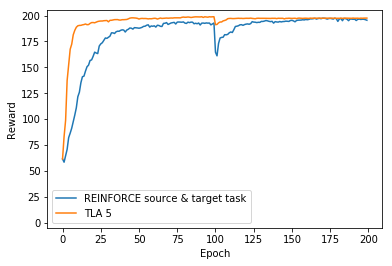
\includegraphics[width=.8\linewidth]{images/results/CartPole/reinforce_2tasks.png}
    \caption{\textit{REINFORCE} applied for 100 epochs to a randomly chosen source task of a \textit{cart-pole} environment and afterwards to the target task, using the same network and weight values.}
    \label{fig:carpole:reward_reinforce_2tasks}
\end{figure}
% subsubsection cart_pole (end)
\subsubsection{Acrobot} % (fold)
\label{ssub:reinforce_source_target:acrobot}
We now do the same experiment for the \textit{acrobot} environment. The resulting learning curve for the source and target task is shown in Figure~\ref{fig:acrobot:reward_reinforce_2tasks}.
\begin{figure}[htb]
    \centering
    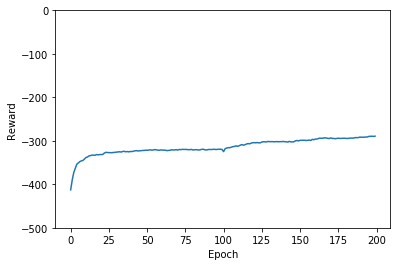
\includegraphics[width=.8\linewidth]{images/results/Acrobot/reinforce_2tasks.png}
    \caption{\textit{REINFORCE} applied for 100 epochs to a randomly chosen source task of an \textit{acrobot} and afterwards to the target task, using the same network and weight values.}
    \label{fig:acrobot:reward_reinforce_2tasks}
\end{figure}
On average, only a small adaption is needed for the target task to reach the same reward as the one with which the source task ended. However, for the target task, the asymptotic performance does not reach the values from our TLA algorithm.
% subsection reinforce_using_a_source_and_target_task (end)
% subsection acrobot (end)

